\clearpage

\def\chaptertitle{Conclusion}

\lhead{\emph{\chaptertitle}}

\chapter{\chaptertitle}
\label{ch:conclusion}

\section{Overview}
\label{sec:ch7-overview}

In conclusion, the thesis provides a novel, lightweight, and SLA-compliant approach to autoscale resources on a micro-service deployed on an edge architecture. In comparison to other state-of-the-art autoscalers, the algorithm performs considerably better in terms of SLA violation as well as resource usage.\par

The autoscaler architecture is open source \footnote{\url{https://github.com/suhridgupta/K8s-Proactive-Forecaster}} \footnote{\url{https://github.com/suhridgupta/jaeger-scraper}}, and provides a framework to further develop more sophisticated auto-scaling solutions. These extensions will be discussed in section \ref{subsec:ch7-extensions}.\par

Furthermore, the outcome of this thesis is being used to develop two publications. The first is a research paper which is aimed to be published in the IEEE Cloud Conference \footnote{\url{https://ieeexplore.ieee.org/xpl/conhome/1002911/all-proceedings}}. The paper will focus on cloud-edge layer deployment of Kubernetes, how the hybrid autoscaler fits into this architecture to provide SLA-compliance, as well as the mathematical modeling of the problem along with the performance evaluation.\par

The second is an implementation framework publication which is aimed to be published in the Future Generation Computer Systems \footnote{\url{https://www.sciencedirect.com/journal/future-generation-computer-systems}} journal. The autoscaler will be presented as an extendable framework on top of Kubernetes. The publication will discuss the modifications made to the autoscaler to make it SLA-compliant, and the methods by which users can develop their own auto-scaling policies using the hybrid autoscaler as a plug-in.\par

\section{Contributions}
\label{sec:ch7-contribution}

The contributions of this thesis can be broken down into three main segments: identifying the major bottlenecks of auto-scaling on an edge deployment in comparison to a typical cloud architecture, designing a novel hybrid auto-scaling architecture which is built primarily of the edge paradigm, and streamlining the forecaster used by the hybrid autoscaler, thus making it capable of running on resource-limited edge deployments.\par

Through the extensive literature review conducted in chapter \ref{ch:lit-review}, the key aspects which make the typical cloud-based hybrid autoscalers infeasible  for edge deployments were identified, this being a lack of computing and storage resources in the edge layer as compared to the cloud layer, the difficulty in hyper-parameter tuning, and the complexity of the forecast models driving up the model training time. With these issues identified, a hybrid auto-scaling architecture was proposed which addressed all the reported bottlenecks, and was capable of scaling resources in the edge environment in an SLA-compliant manner.\par

Based on the investigation of existing hybrid autoscalers conducted in section \ref{sec:ch3-hybrid-solutions}, all existing autoscalers are not edge architecture compliant, as they were too resource intensive, or not SLA-compliant, or both. Thus the hybrid architecture proposed in this thesis was a novel approach which maintained SLA compliance and ease-of-deployment on edge paradigms. It did so by combining a reactive autoscaler with a streamlined proactive model built using LSTM. To eliminate the difficult hyper-parameter tuning process, the autoscaler was built with a heuristic approach in mind, where the parameters were automatically fine-tuned in case any SLA violations were seen in the data.\par

Finally, the autoscaler was tested on a production-ready social network micro-service deployment, and the results were compared with other cutting-edge autoscalers. The results showed that the proposed autoscaler has a maximum SLA violation rate of $5.41\%$, as compared to a maximum of $18.8-22.38\%$ for the other state-of-the-art autoscalers.\par

The tests were further able to demonstrate that the autoscaler was capable of significantly reducing SLA violations while also keeping the overall cost related to deploying the container orchestration resources on a cloud provider as low as possible. It does so by assigning resources in a manner which keeps the utilized resources at approximately half of the configured auto-scaling threshold.\par

Based on the work done in this thesis, the research questions stated in section \ref{sec:ch1-problem-overview} can be conclusively answered.

\begin{itemize}
    \item \textbf{\textit{RQ1:}} The work done in this thesis successfully integrated reactive and proactive auto-scaling algorithms to develop a hybrid autoscaler tailored for edge computing architectures. The autoscaler was both light weight, allowing it to be run on the edge layer, while also eliminating the requirement for tedious and complicated hyper-parameter tuning seen in most proactive auto-scaling solutions.
    \item \textbf{\textit{RQ2:}} The work done in this thesis successfully demonstrated that the autoscaler exceeded the SLA compliance capabilities of state-of-the-art reactive and proactive auto-scaling solutions for edge computing, while minimizing the cost of deploying the application.
\end{itemize}

\section{Future Work}
\label{sec:ch7-future-work}

\subsection{Current Limitations}
\label{subsec:ch7-limitations}

Several assumptions have been made when conducting the experiments, the primary ones being that only a single SLA metric was used to design the heuristic model, the auto-scaling approach was limited to horizontally scaling resources, and the forecaster used a simple LSTM machine learning model using a single parameter. In the next section, some extensions to improve the robustness of the hybrid autoscaler is proposed, along with some approaches to improve the efficiency and accuracy of its forecasts.\par

\subsection{Proposed Extensions}
\label{subsec:ch7-extensions}

\subsubsection{Alternative Auto-scaling Approaches}
\label{subsubsec:ch7-alternate-auto}

The proposed hybrid model autoscales resources in a strictly horizontal manner. One of the underlying assumptions was that no other auto-scaling was to take place while the micro-service deployments were being stress tested. This meant that only the number of deployment replicas were either increased or decreased, keeping all other parameters untouched.\par

A future extension to this thesis would be to configure the algorithm such that it can attempt other forms of auto-scaling too. For example, the hybrid model may be configured as a Vertical Pod Autoscaler (VPA) instead. In this approach, the reactive autoscaler will modify the CPU reservations for the deployments, while leaving the number of deployment replicas untouched. Similarly, the proactive forecaster will attempt to predict the future CPU workload, and autoscale beforehand accordingly. The benefit of such an approach is that the forecaster already works in a similar manner, predicting future CPU workloads, and thus only minor modifications would be required to configure the hybrid HPA into a VPA.\par

A more challenging extension would be to transform the hybrid model into a Cluster Autoscaler. In the cluster autoscaler, the container orchestration platform will adjust the size of the cluster (edge nodes) when one of the following conditions holds:

\begin{itemize}
    \item There are deployment replicas in the cluster which are currently un-assigned to any node due to insufficient resources.
    \item There are nodes in the cluster that have not had sufficient utilization of resources for a configured period of time, and as such, their active deployment replicas can be re-scheduled on to other nodes, after which the node can be decommissioned to free up resources.
\end{itemize}

While converting this autoscaler architecture for cloud computing is a straightforward process, due to the inherent homogeneity of the paradigm, it is much more difficult for an edge computing approach. Since different resource workloads are exerted on the various edge nodes, care needs to be taken when re-scheduling deployment replicas to other nodes, as well as decommissioning nodes. This process needs to be done in an intelligent manner such that the overall latency of the micro-service does not increase due to an added distance between the end user and the modified edge layer architecture. Therefore the auto-scaling controller must be modified in a way such that it can identify nodes nearby to it such that it can re-assign replicas.

\subsubsection{Multi-Variate Forecaster}
\label{subsubsec:ch7-multi-variate}

The forecaster used in the hybrid autoscaler is a uni-variate LSTM model. This means that at any given time, only one variable is changing. Therefore the input is a one-dimensional array. An extension can be made to the forecaster to convert it into a multi-variate model. In this approach, multiple variables are being modified at a given time, thus the input to the model is a more complex two-dimensional array.\par

The benefit of a multi-variate approach is that a more holistic auto-scaling decision can be made using this. For example, the VPA model discussed in section \ref{subsubsec:ch7-alternate-auto}, the reactive and proactive algorithms can be modified to autoscale on both CPU and memory utilization. The forecaster can then take the CPU and memory time-series data as input, and output the forecast for both. Through this, the autoscaler can form a better picture of the resource utilization of the micro-service, identifying bottlenecks and mitigating them.\par

The drawback of such an approach is that the proactive forecaster training times will significantly increase due to two reasons. The first one is the additional complexity of the input as well as output. Due to the multiple variables needing to be trained and validated on, more epochs are required, along with each epoch taking longer to evaluate. Furthermore the validation process will take longer as well. The second cause is due to the memory time-series not being as predictable as the CPU utilization. In the CPU utilization graphs of the deployments as seen in figure \ref{fig:lstm-init-data}, the workload forms clear and identifiable patterns which can be easily recognized by the model. Memory is far more variable, with sudden peaks and falls depending on several of the processes running in the deployment. Thus the autoscaler must concomitantly be made as complex, with far larger and deeper neural network architectures.\par

Due to this drawback, further research is required to verify the feasibility of using a multi-variate machine learning model to forecast workloads, and to confirm whether or not it is suitable for an edge deployment.

\begin{comment}
\subsubsection{Auto-regressive Forecaster}
\label{subsubsec:ch7-auto-regressive}

So far, the proactive forecaster implemented in the hybrid solution, along with the enhancements discussed above, have predicted the entire output in a single step. There is an alternative method of forecasting, where the model decomposes this prediction process into individual steps. By doing so, at each step the model's outputs can be fed back into itself, making the next prediction dependant on the output of the previous one. Figure \ref{fig:auto-regressive-lstm} shows a simplified overview of this process.\par

\begin{figure}[htb]
    \centering
    \caption{Auto-Regressive LSTM Prediction, courtesy of Tensorflow \cite{autoregressivelstm}}
    \label{fig:auto-regressive-lstm}
    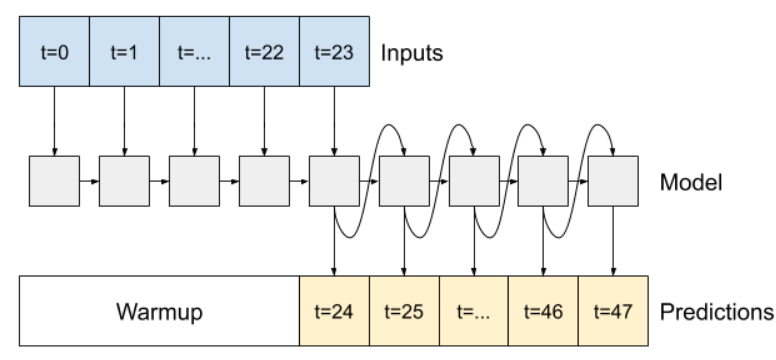
\includegraphics[width=0.6\linewidth]{Figures/Auto-Regressive-LSTM.png}
\end{figure}

There are benefits in using an auto-regressive approach, the training window, which is the number of previous steps which the LSTM model uses to predict the output, can be drastically lowered for large outputs. This is because the model is no longer predicting a large output in one shot, but unit predictions in an iterative process. Another benefit is that the model can re-use the previously predicted data as training input for the subsequent prediction steps, which can potentially increase the accuracy of the model. Lastly, this model is highly customizable. Whereas the hybrid approach proposed in this algorithm predicts 24 hours of data points, the auto-regressive approach can be set to output predictions of any length.\par

However this added complexity requires far larger usage of resources. Furthermore, the iterative prediction process can result in a lack of parallel resource usage, meaning it takes far longer to predict the same amount of data as seen in proposed hybrid solution. Further research is required to verify if such an auto-regressive model is feasible for an edge deployment.
\end{comment}

\subsubsection{Multi-SLA Constraints}
\label{subsubsec:ch7-multi-sla}

Another modification which can be made to the hybrid autoscaler is to support the use of multiple SLA constraints. Currently, the autoscaler only takes into account a single metric, and bases its heuristic feedback algorithm on it. By modifying this into a multi-parameter model, the autoscaler can keep a track of several metrics, and if a violation occurs on any one of them, can tune the auto-scaling process accordingly.\par

Such a modification opens up several other possibilities too. Each SLA metric can be given its own weight to denote importance. The current hybrid autoscaler only considers a single action of tuning the forecaster hyper-parameter variables on SLA violation occurrences. By making it a multi-SLA model with different weights attached, the hybrid autoscaler can intelligently decide what actions to take when on different scenarios such as urgent and mild SLA violations.\par

This adds further complexity to the autoscaler however, and the constant tuning of forecast parameters may cause issues such as a drop in prediction accuracy and under-fitting / over-fitting. Thus a balance needs to be struck in the actions to be taken on SLA constraints being violated, and additional cooldowns need to be implemented on the frequency of such actions being implemented.

\begin{comment}
\subsubsection{Alternative LSTM Configurations}
\label{subsubsec:ch7-advanced-lstm-config}

A \textit{classic LSTM} model, similar to the one implemented by Hochreiter and Schmidhuber \cite{hochreiter1997long} was used in this research. As explained in section \ref{sec:ch2-time-series}, this consists of memory cells, forget gates, input gates, and output gates. The strength of such a model lies in its ability to extract features from the data with varying time lags to create long-range dependencies. This model however has several extensions, some of which are discussed below.\par

\textit{Bidirectional LSTM} \cite{graves2005framewise} is an extension of the classic LSTM architecture. This model encompasses bi-directional processing to enable the capture of information from both the past and future inputs. This is done using two separate LSTM layers, a forward LSTM layer which processes the input from beginning to end, and a backward LSTM layer which processes the input in reverse. The outputs of both layers are concatenated at each step, thus capturing a richer feature set from the data to make a more accurate forecast. This approach is resource intensive, however, and may see limited improvements over the classic approach, since Bidirectional LSTM models are best suited for applications where understanding the sequential context in both directions is crucial \cite{breuel2015benchmarking}.\par

\textit{LSTM with attention mechanisms} \cite{zheng2021understanding} transforms the classic LSTM to allow the model to focus on specific features of the data. This architecture incorporates attention weights that compute the importance of each input at a given training iteration. These attention weights are adjusted dynamically during the training process based on the relevance of each input element for the current prediction. By focusing on specific sections of the input, the model can better capture dependencies in lengthy input data series without being overwhelmed, resulting in higher prediction accuracy \cite{zhou2020comparison}. There are some drawbacks to applying such an approach to an edge micro-service however, since this model is best used for capturing fine-grained dependencies in the time-series data. Such detailed dependencies are not required in a hybrid model, since the reactive portion of the autoscaler can shoulder most of the auto-scaling responsibility. Thus further research needs to be carried out in evaluating the benefits of using such a proactive forecaster approach.\par

Finally, a model which may provide faster training times is the \textit{Gated Recurrent Unit} (GRU) \cite{chung2014empirical}. The GRU combines the input and forget gates of the classic LSTM into a unified gate. Similarly, the cell state and hidden output are also combined into a combined hidden state layer. Finally, the model contains an internal hidden state. Through these modifications, the GRU is able to efficiently capture dependencies and features in sequential data, making them particularly useful for resource-constrained real-time applications, such as edge deployments \cite{yang2020lstm}. Using this model may eliminate some of the performance drawbacks seen in multi-variate forecasters in section \ref{subsubsec:ch7-multi-variate} making it a viable alternative for implementing such a system.\par
\end{comment}